% Chapter 7

\chapter{The second wire, induced interaction} % Main chapter title

\label{Chapter8} % For referencing the chapter elsewhere, use \ref{Chapter8} 

\lhead{Chapter 8. \emph{The 2nd wire, induced interaction}} % This is for the header on each page - perhaps a shortened title

%----------------------------------------------------------------------------------------
In the chapter we will introduce a second wire parallel to the first one already studied. The aim here is to calculate the additional (interwire) induced interaction between the wires. The approach mirrors chapter \ref{Chapter3}. For this reason we will not go in as much detail in the present chapter.
\section{The effective Bose-Fermi interaction} 
As for the single wire the effective Bose-Fermi interaction is modelled by $V(\mathbf{r}) = g_{BF}\delta(\mathbf{r})$. To begin with, this gives the same expression for the interaction Hamiltonian between the bosons (B) and the fermions (F):
\begin{equation}
H_{BF}^\text{int} = g_{BF}\int d^3 r \hat{\psi}_F^\dagger(\mathbf{r}) \hat{\psi}_B^\dagger(\mathbf{r})\hat{\psi}_B(\mathbf{r})\hat{\psi}_F(\mathbf{r}).
\end{equation}

The difference now is, that we trap the fermions along \textit{two} wires. Let the first one be along the $x$-axis, the second at $z=d, y=0$. The fermions are trapped in a harmonic trap with trapping frequency $\omega_t$. In this connection we have two central assumptions. The first is the same as for the single wire: we require, that the fermions are trapped in the ground state with respect to the perpendicular directions. The second assumption is, that the distance between the wires is much larger than the trapping width of the wires $l_t = \frac{1}{\sqrt{m_F\omega_t}}$. Hence, $l_t/d \gg 1$. This is done, so that we can actually talk about distinguishable wires of fermions. This leads to the following expansion in momentum eigenstates:
\begin{equation}
\psi_F(x,\mathbf{r}_\perp) = \frac{1}{\sqrt{\mathcal{L}}}\sum_p \text{e}^{ipx} \left[\phi_0(\mathbf{r}_\perp) f_{1,p} + \phi_0(\mathbf{r}_\perp-\mathbf{d}) f_{2,p}\right], \hspace{0.5cm} \psi_B(\mathbf{r}) = \frac{1}{\sqrt{\mathcal{V}}}\sum_{\mathbf{k}} \text{e}^{i\mathbf{k}\cdot \mathbf{r}} b_\mathbf{k}, 
\end{equation}  
with $\phi_0(\mathbf{r}_\perp) = \frac{1}{\sqrt{\pi}l_t}\exp\left(-\frac{r_\perp^2}{2l_t^2}\right)$ the ground state with respect to the perpendicular directions. $f^\dagger_{j,p}$ therefore creates a fermion in wire $j$ with momentum $p$. We assume, that the wires are truly distinguishable. This means that all anticommutators like $\{f_{1,p}, f^\dagger_{2,p'}\}$ vanish. Inserting these expressions into $H_{BF}^\text{int}$ yields in total four terms. However, the cross terms where a fermion is annihilated in one wire and created in the other are proportional to the integral:
\begin{equation}
\int d^2 r_\perp \phi_0(\mathbf{r}_\perp)\phi_0(\mathbf{r}_\perp-\mathbf{d}) = 0. 
\end{equation}
The integral is negligible, because by assumption $l_t/d \gg 1$. A similar analysis to the one in chapter \ref{Chapter3} then yields for the diagonal terms:
\begin{align}
H_{BF}^\text{int} = \frac{g_{BF}}{\mathcal{V}}\sum_{p_1,p_2,q} \sum_{\mathbf{k}_\perp, \mathbf{k}_\perp'} & \text{e}^{-\frac{l_t^2}{4}(\mathbf{k}_\perp - \mathbf{k}_\perp')^2}\left[ f^\dagger_{1,p_2-q} b^\dagger_{p_1+q, \mathbf{k}_\perp'} b_{p_1,\mathbf{k}_\perp}f_{1,p_2} + \right. \nonumber \\
& \left. \text{e}^{i(\mathbf{k}_\perp - \mathbf{k}_\perp')\cdot \mathbf{d}}f_{2,p_2-q}^\dagger b_{p_1+q, \mathbf{k}_\perp'}^\dagger b_{p_1,\mathbf{k}_\perp}f_{2,p_2} \right].
\end{align}

This shows, that a scattering event in wire 1 is associated with the factor $g_{BF} \text{e}^{-\frac{l_t^2}{4}(\mathbf{k}_\perp - \mathbf{k}_\perp')^2}$ as before, and that the corresponding scattering in wire 2 has an extra factor of $\text{e}^{i(\mathbf{k}_\perp - \mathbf{k}_\perp')\cdot \mathbf{d}}$. 

\section{The 1D-3D induced interaction}
The intrawire induced interaction is (of course) the same as the one for the single line. Referring to equation \ref{eq.VFFindXBEC} this means, that:
\begin{equation}
V_{FF,11}^\text{ind}(q,i\omega_q) = V_{FF,22}^\text{ind}(q,i\omega_q) = g_{BF}^2\int\frac{d^2k_\perp}{(2\pi)^2}\; \chi_\text{BEC}(q,\mathbf{k}_\perp,i\omega_q)\text{e}^{-\frac{l_t^2}{2}k_\perp^2}, 
\label{eq.VFF1122indXBEC} 
\end{equation}
with $\chi_\text{BEC}(\mathbf{k},i\omega_q) = \frac{k^2}{m_B}\frac{n_B}{(i\omega_q)^2-E_{B,k}^2}$ the density-density correlation function. The index $11$ ($22$) indicates, that the interaction is between two fermions in wire 1 (wire 2). One might wonder what happens to the extra factor of $\text{e}^{i(\mathbf{k}_\perp - \mathbf{k}_\perp')\cdot \mathbf{d}}$. The incoming boson is associated with a factor of $\text{e}^{i\mathbf{k}_\perp\cdot \mathbf{d}}$. However, the outgoing is associated with a factor of $\text{e}^{-i\mathbf{k}_\perp\cdot \mathbf{d}}$, and so these cancel. This is as it should be, because the intrawire interaction in the two wires should be the same!

The additional scenario now is, that there is also an interwire induced interaction, which we will denote $V_{FF,12}^\text{ind}(q,i\omega_q)$. The preceding section shows, that the calculation of this induced interaction is analogous to the above, but with the additional factor of $\text{e}^{i\mathbf{k}_\perp\cdot \mathbf{d}}$ from scattering in the second wire. Explicitly the Feynman diagrams of importance are shown in figure \ref{fig.interwirefeynmandiagrams}. They have the same form as the ones in figure \ref{fig.feynmandiagrams} with the (obvious) caveat, that the induced interaction is now between a fermion in wire 1 and a fermion in wire 2. Hence,
\begin{equation}
V_{FF,12}^\text{ind}(q,i\omega_q) = g_{BF}^2\int\frac{d^2k_\perp}{(2\pi)^2}\; \chi_\text{BEC}(q,\mathbf{k}_\perp,i\omega_q)\text{e}^{-\frac{l_t^2}{2}k_\perp^2}\text{e}^{i\mathbf{k}_\perp\cdot \mathbf{d}}. 
\label{eq.VFF12indXBEC} 
\end{equation}

\begin{figure}
\begin{tikzpicture}[scale=0.25]
  \begin{feynman}[small]
    \vertex (number1) {\( (1) \)};
    \vertex [above left=of number1] (fermion1) {\( 1, \tilde{p}_1 \)};
    \vertex [above right=of fermion1] (a);
    \vertex [below right=of a] (fermion2) {\(1, \tilde{p}_1+\tilde{q}\)}; 
    \vertex [above=of a] (b);
    \vertex [left=of b] (boson1) {\( \sqrt{n_B} \)}; 
    \vertex [above= of b] (c);
    \vertex [right= of c] (boson2) {\( \sqrt{n_B} \)};
    \vertex [above= of c] (d);
    \vertex [above left=of d] (f3) {\(2, \tilde{p}_2\)};
    \vertex [above right=of d] (f4) {\(2, \tilde{p}_2-\tilde{q}\)};
 
    \diagram* {
      (number1) -- [opacity=0.0] (fermion1) -- [fermion] (a) -- [fermion] (fermion2),
      (a) -- [photon, edge label'=\(g_{BF}\)] (b),
      (b) -- [dashed] (boson1),
      (b) -- [blue, fermion, edge label' = {\(-\tilde{q}, \mathbf{k}_\perp \)}] (c),
      (c) -- [dashed] (boson2),
      (c) -- [photon, edge label'=\(g_{BF}\)] (d),
      (d) -- [anti fermion] (f3),
      (d) -- [fermion] (f4)
    };
  \end{feynman}
\end{tikzpicture}
\begin{tikzpicture}
  \begin{feynman}[small]
    \vertex (number2) {\( (2) \)};
    \vertex [above left=of number2] (fermion1) {\(1, \tilde{p}_1 \)};
    \vertex [above right=of fermion1] (a);
    \vertex [below right=of a] (fermion2) {\(1, \tilde{p}_1+\tilde{q}\)}; 
    \vertex [above=of a] (b);
    \vertex [left=of b] (boson1) {\( \sqrt{n_B} \)}; 
    \vertex [above= of b] (c);
    \vertex [right= of c] (boson2) {\( \sqrt{n_B} \)};
    \vertex [above= of c] (d);
    \vertex [above left=of d] (f3) {\(2, \tilde{p}_2\)};
    \vertex [above right=of d] (f4) {\(2, \tilde{p}_2-\tilde{q}\)};
 
    \diagram* {
      (number2) -- [opacity=0.0] (fermion1) -- [fermion] (a) -- [fermion] (fermion2),
      (a) -- [photon, edge label'=\(g_{BF}\)] (b),
      (b) -- [dashed] (boson1),
      (b) -- [blue, anti fermion, edge label' = {\(\tilde{q}, \mathbf{k}_\perp \)}] (c),
      (c) -- [dashed] (boson2),
      (c) -- [photon, edge label'=\(g_{BF}\)] (d),
      (d) -- [anti fermion] (f3),
      (d) -- [fermion] (f4)
    };
  \end{feynman}
\end{tikzpicture}
\begin{tikzpicture}
  \begin{feynman}[small]
    \vertex (number3) {\( (3) \)};
    \vertex [above left=of number3] (fermion1) {\(1, \tilde{p}_1 \)};
    \vertex [above right=of fermion1] (a);
    \vertex [below right=of a] (fermion2) {\(1, \tilde{p}_1+\tilde{q}\)}; 
    \vertex [above=of a] (b);
    \vertex [left=of b] (boson1) {\( \sqrt{n_B} \)}; 
    \vertex [above= of b] (c);
    \vertex [right= of c] (boson2) {\( \sqrt{n_B} \)};
    \vertex [above= of c] (d);
    \vertex [above left=of d] (f3) {\(2, \tilde{p}_2\)};
    \vertex [above right=of d] (f4) {\(2, \tilde{p}_2-\tilde{q}\)};
 
    \diagram* {
      (number3) -- [opacity=0.0] (fermion1) -- [fermion] (a) -- [fermion] (fermion2),
      (a) -- [photon, edge label'=\(g_{BF}\)] (b),
      (b) -- [dashed] (boson1),
      (b) -- [blue, majorana, edge label' = {\(\tilde{q}, \mathbf{k}_\perp \)}] (c),
      (c) -- [dashed] (boson2),
      (c) -- [photon, edge label'=\(g_{BF}\)] (d),
      (d) -- [anti fermion] (f3),
      (d) -- [fermion] (f4)
    };
  \end{feynman}
\end{tikzpicture}
\begin{tikzpicture}
  \begin{feynman}[small]
    \vertex (number4) {\( (4) \)};
    \vertex [above left=of number4] (fermion1) {\(1, \tilde{p}_1 \)};
    \vertex [above right=of fermion1] (a);
    \vertex [below right=of a] (fermion2) {\(1, \tilde{p}_1+\tilde{q}\)}; 
    \vertex [above=of a] (b);
    \vertex [left=of b] (boson1) {\( \sqrt{n_B} \)}; 
    \vertex [above= of b] (c);
    \vertex [right= of c] (boson2) {\( \sqrt{n_B} \)};
    \vertex [above= of c] (d);
    \vertex [above left=of d] (f3) {\(2, \tilde{p}_2\)};
    \vertex [above right=of d] (f4) {\(2, \tilde{p}_2-\tilde{q}\)};
 
    \diagram* {
      (number3) -- [opacity=0.0] (fermion1) -- [fermion] (a) -- [fermion] (fermion2),
      (a) -- [photon, edge label'=\(g_{BF}\)] (b),
      (b) -- [dashed] (boson1),
      (b) -- [blue, anti majorana, edge label' = {\(\tilde{q}, \mathbf{k}_\perp \)}] (c),
      (c) -- [dashed] (boson2),
      (c) -- [photon, edge label'=\(g_{BF}\)] (d),
      (d) -- [anti fermion] (f3),
      (d) -- [fermion] (f4)
    };
  \end{feynman}
\end{tikzpicture}
\caption{Feynman diagrams for the induced interaction between the wires. Since the interaction is weak, we can neglect all other Feynman diagrams than (1)-(4). Diagrams (1) and (2) stems from the normal Green's function $G_{11}$. Diagrams (3) and (4) stems from the anormalous Green's function $G_12$.} \label{fig.interwirefeynmandiagrams}
\end{figure}


We will in only investigate the $l_t \to 0$ and $\omega_q = 0$ limit. The reasoning behind the $\omega_q = 0$ limit is the same as for the single wire. See \ref{sec.RetardationEffects} for details. Further, it is already here possible to take the $l_t \to 0$ limit in contrast to the intrawire interaction case. By rewriting the above integral, we get:
\begin{align}
V_{FF,12}^\text{ind}(q,0) &= -\frac{n_Bg_{BF}^2m_B}{\pi^2}\int_0^\infty d k_\perp \; \frac{k_\perp}{k_\perp^2 + q^2 + 2/\xi^2} \int_0^{2\pi} d\theta \; \text{e}^{ik_\perp d\cos(\theta)} \nonumber \\
						  &= -\frac{2n_Bg_{BF}^2m_B}{\pi}\int_0^\infty d k_\perp \; \frac{k_\perp J_0(k_\perp d)}{k_\perp^2 + q^2 + 2/\xi^2},
\label{eq.secondwireinducedinteractionmomentumspaceintegralexpression}
\end{align}
with $J_0$ is the zero order Bessel function of the first kind. This form of the potential is not terrible illuminating. In stead let us take the Fourier transform to get the induced interaction in real space, $\tilde{V}^\text{ind}_{FF}(x,0)$. Write $\mathbf{r} = (x,\mathbf{d})$ and $\mathbf{k} = (q,\mathbf{k}_\perp)$. We then get the expression:
\begin{align}
\tilde{V}_{FF,12}^\text{ind}(x,0) &= \int \frac{dq}{2\pi} \; \text{e}^{iqx} V_{FF,12}^\text{ind}(q,0) = -4n_Bg^2_{BF}m_B\int \frac{d^3k}{(2\pi)^3} \frac{\text{e}^{i\mathbf{k}\cdot \mathbf{r}}}{k^2 + 2/\xi^2} \nonumber \\
								  &= -\frac{n_Bg^2_{BF}m_B}{\pi} \frac{\text{e}^{-\sqrt{2(x^2+d^2)}/\xi}}{\sqrt{x^2+d^2}},
\end{align}
since we recognise the second expression as the Yukawa potential in momentum space with range $\sqrt{2}/\xi$. The interwire induced interaction is hereby shown to be the natural generalisation of the intrawire interaction found in chapter \ref{Chapter3}. This further enables us to get a closed form expression for the induced interaction in momentum space. Writing up the Fourier transform, we get:
\begin{equation}
V^\text{ind}_{FF,12}(q,0) = \int dx \; \text{e}^{-iqx}\tilde{V}^\text{ind}_{FF,12}(x,0) = 2\int_0^\infty \cos(qx)\tilde{V}^\text{ind}_{FF,12}(x,0), \nonumber 
\end{equation}
since the induced interaction is even in real space. Writing the variables in units of the range $\sqrt{2}/\xi$, we get:
\begin{equation}
V^\text{ind}_{FF,12}(\tilde{q},0) = -\frac{2n_Bg^2_{BF}m_B}{\pi}\int_0^\infty d\tilde{x} \cos(\tilde{q}\tilde{x})\frac{ \text{e}^{ -\sqrt{\tilde{x}^2+\tilde{d}^2} } }{\sqrt{\tilde{x}^2+\tilde{d}^2}} = -\frac{2n_Bg^2_{BF}m_B}{\pi}K_0\left(\tilde{d}\sqrt{\tilde{q}^2+1}\right), \nonumber
\end{equation}
where $K_0(x)$ is the modified Bessel function of the second kind of order zero. This calculation is done with the use of the Fourier cosine transform routine in Maple 16. The result is verified by comparing it graphically to the integral expression of equation \eqref{eq.secondwireinducedinteractionmomentumspaceintegralexpression}. Since $\tilde{q} = \frac{q\xi}{\sqrt{2}}, \tilde{d} = \frac{\sqrt{2}d}{\xi}$, we finally get:
 \begin{equation}
V^\text{ind}_{FF,12}(q,0) = -\frac{2n_Bg^2_{BF}m_B}{\pi}K_0\left(\sqrt{(qd)^2+\frac{2d^2}{\xi^2}}\right). 
\end{equation}
The fact, that we can express the induced interaction in terms of a known function is crucial for the feasibility of the later numerical analysis. 

\begin{figure} 
\begin{center}  
% GNUPLOT: LaTeX picture with Postscript
\begingroup
  \makeatletter
  \providecommand\color[2][]{%
    \GenericError{(gnuplot) \space\space\space\@spaces}{%
      Package color not loaded in conjunction with
      terminal option `colourtext'%
    }{See the gnuplot documentation for explanation.%
    }{Either use 'blacktext' in gnuplot or load the package
      color.sty in LaTeX.}%
    \renewcommand\color[2][]{}%
  }%
  \providecommand\includegraphics[2][]{%
    \GenericError{(gnuplot) \space\space\space\@spaces}{%
      Package graphicx or graphics not loaded%
    }{See the gnuplot documentation for explanation.%
    }{The gnuplot epslatex terminal needs graphicx.sty or graphics.sty.}%
    \renewcommand\includegraphics[2][]{}%
  }%
  \providecommand\rotatebox[2]{#2}%
  \@ifundefined{ifGPcolor}{%
    \newif\ifGPcolor
    \GPcolortrue
  }{}%
  \@ifundefined{ifGPblacktext}{%
    \newif\ifGPblacktext
    \GPblacktexttrue
  }{}%
  % define a \g@addto@macro without @ in the name:
  \let\gplgaddtomacro\g@addto@macro
  % define empty templates for all commands taking text:
  \gdef\gplbacktext{}%
  \gdef\gplfronttext{}%
  \makeatother
  \ifGPblacktext
    % no textcolor at all
    \def\colorrgb#1{}%
    \def\colorgray#1{}%
  \else
    % gray or color?
    \ifGPcolor
      \def\colorrgb#1{\color[rgb]{#1}}%
      \def\colorgray#1{\color[gray]{#1}}%
      \expandafter\def\csname LTw\endcsname{\color{white}}%
      \expandafter\def\csname LTb\endcsname{\color{black}}%
      \expandafter\def\csname LTa\endcsname{\color{black}}%
      \expandafter\def\csname LT0\endcsname{\color[rgb]{1,0,0}}%
      \expandafter\def\csname LT1\endcsname{\color[rgb]{0,1,0}}%
      \expandafter\def\csname LT2\endcsname{\color[rgb]{0,0,1}}%
      \expandafter\def\csname LT3\endcsname{\color[rgb]{1,0,1}}%
      \expandafter\def\csname LT4\endcsname{\color[rgb]{0,1,1}}%
      \expandafter\def\csname LT5\endcsname{\color[rgb]{1,1,0}}%
      \expandafter\def\csname LT6\endcsname{\color[rgb]{0,0,0}}%
      \expandafter\def\csname LT7\endcsname{\color[rgb]{1,0.3,0}}%
      \expandafter\def\csname LT8\endcsname{\color[rgb]{0.5,0.5,0.5}}%
    \else
      % gray
      \def\colorrgb#1{\color{black}}%
      \def\colorgray#1{\color[gray]{#1}}%
      \expandafter\def\csname LTw\endcsname{\color{white}}%
      \expandafter\def\csname LTb\endcsname{\color{black}}%
      \expandafter\def\csname LTa\endcsname{\color{black}}%
      \expandafter\def\csname LT0\endcsname{\color{black}}%
      \expandafter\def\csname LT1\endcsname{\color{black}}%
      \expandafter\def\csname LT2\endcsname{\color{black}}%
      \expandafter\def\csname LT3\endcsname{\color{black}}%
      \expandafter\def\csname LT4\endcsname{\color{black}}%
      \expandafter\def\csname LT5\endcsname{\color{black}}%
      \expandafter\def\csname LT6\endcsname{\color{black}}%
      \expandafter\def\csname LT7\endcsname{\color{black}}%
      \expandafter\def\csname LT8\endcsname{\color{black}}%
    \fi
  \fi
    \setlength{\unitlength}{0.0500bp}%
    \ifx\gptboxheight\undefined%
      \newlength{\gptboxheight}%
      \newlength{\gptboxwidth}%
      \newsavebox{\gptboxtext}%
    \fi%
    \setlength{\fboxrule}{0.5pt}%
    \setlength{\fboxsep}{1pt}%
\begin{picture}(7200.00,5040.00)%
    \gplgaddtomacro\gplbacktext{%
      \csname LTb\endcsname%
      \put(682,767){\makebox(0,0)[r]{\strut{}$-5$}}%
      \csname LTb\endcsname%
      \put(682,1609){\makebox(0,0)[r]{\strut{}$-4$}}%
      \csname LTb\endcsname%
      \put(682,2451){\makebox(0,0)[r]{\strut{}$-3$}}%
      \csname LTb\endcsname%
      \put(682,3292){\makebox(0,0)[r]{\strut{}$-2$}}%
      \csname LTb\endcsname%
      \put(682,4134){\makebox(0,0)[r]{\strut{}$-1$}}%
      \csname LTb\endcsname%
      \put(682,4976){\makebox(0,0)[r]{\strut{}$0$}}%
      \csname LTb\endcsname%
      \put(1463,484){\makebox(0,0){\strut{}$-4$}}%
      \csname LTb\endcsname%
      \put(2636,484){\makebox(0,0){\strut{}$-2$}}%
      \csname LTb\endcsname%
      \put(3809,484){\makebox(0,0){\strut{}$0$}}%
      \csname LTb\endcsname%
      \put(4981,484){\makebox(0,0){\strut{}$2$}}%
      \csname LTb\endcsname%
      \put(6154,484){\makebox(0,0){\strut{}$4$}}%
    }%
    \gplgaddtomacro\gplfronttext{%
      \csname LTb\endcsname%
      \put(176,2871){\rotatebox{-270}{\makebox(0,0){\strut{}$2m_F/k_F V_{FF,12}^\text{ind}(q,0)$}}}%
      \put(3808,154){\makebox(0,0){\strut{}$q/k_F$}}%
      \csname LTb\endcsname%
      \put(2197,1600){\makebox(0,0)[r]{\strut{}$k_Fd = 1.8$}}%
      \csname LTb\endcsname%
      \put(2197,1380){\makebox(0,0)[r]{\strut{}$k_Fd = 1.4$}}%
      \csname LTb\endcsname%
      \put(2197,1160){\makebox(0,0)[r]{\strut{}$k_Fd = 1.0$}}%
      \csname LTb\endcsname%
      \put(2197,940){\makebox(0,0)[r]{\strut{}$k_Fd = 0.6$}}%
    }%
    \gplbacktext
    \put(0,0){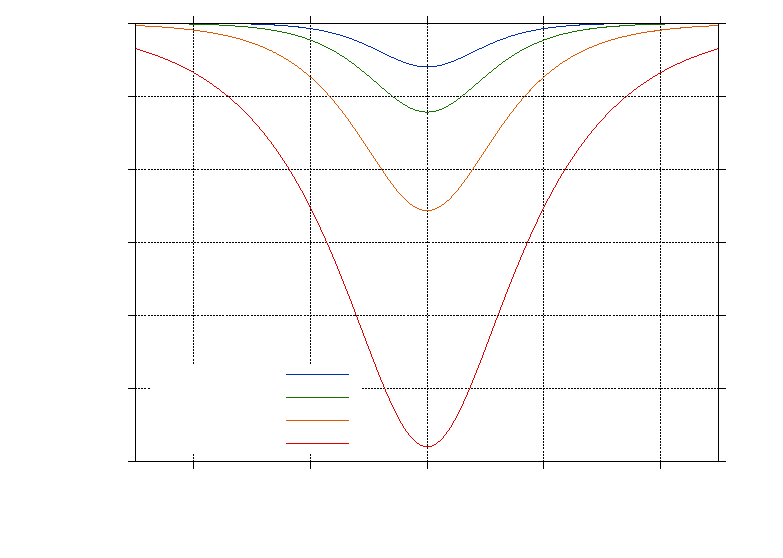
\includegraphics{Figures/twowires/InducedInteractionInterwireMomentumSpace/InducedInteraction}}%
    \gplfronttext
  \end{picture}%
\endgroup
  
\caption{The zero frequency potential $V_{FF,12}^\text{ind}(q,0)$ plotted as a function of $q$. The induced interaction is seen to increase with decreasing distance $d$. Parameters: $(n_Ba_B^3)^{1/3} = 0.01$, $(n_Ba_{BF}^3)^{1/3} = 0.1$, $l_t = 0$, $\frac{m_B}{m_F} = 7/40$, $\frac{n_F}{n_B^{1/3}} = 0.215$, $\frac{m_F^2}{m_B^2}\frac{n_B}{n_F^3} k_Fa_B = 22.10$.}  
\label{fig.VFF12indq}  
\end{center}    
\end{figure}

\begin{figure} 
\begin{center}  
% GNUPLOT: LaTeX picture with Postscript
\begingroup
  \makeatletter
  \providecommand\color[2][]{%
    \GenericError{(gnuplot) \space\space\space\@spaces}{%
      Package color not loaded in conjunction with
      terminal option `colourtext'%
    }{See the gnuplot documentation for explanation.%
    }{Either use 'blacktext' in gnuplot or load the package
      color.sty in LaTeX.}%
    \renewcommand\color[2][]{}%
  }%
  \providecommand\includegraphics[2][]{%
    \GenericError{(gnuplot) \space\space\space\@spaces}{%
      Package graphicx or graphics not loaded%
    }{See the gnuplot documentation for explanation.%
    }{The gnuplot epslatex terminal needs graphicx.sty or graphics.sty.}%
    \renewcommand\includegraphics[2][]{}%
  }%
  \providecommand\rotatebox[2]{#2}%
  \@ifundefined{ifGPcolor}{%
    \newif\ifGPcolor
    \GPcolortrue
  }{}%
  \@ifundefined{ifGPblacktext}{%
    \newif\ifGPblacktext
    \GPblacktexttrue
  }{}%
  % define a \g@addto@macro without @ in the name:
  \let\gplgaddtomacro\g@addto@macro
  % define empty templates for all commands taking text:
  \gdef\gplbacktext{}%
  \gdef\gplfronttext{}%
  \makeatother
  \ifGPblacktext
    % no textcolor at all
    \def\colorrgb#1{}%
    \def\colorgray#1{}%
  \else
    % gray or color?
    \ifGPcolor
      \def\colorrgb#1{\color[rgb]{#1}}%
      \def\colorgray#1{\color[gray]{#1}}%
      \expandafter\def\csname LTw\endcsname{\color{white}}%
      \expandafter\def\csname LTb\endcsname{\color{black}}%
      \expandafter\def\csname LTa\endcsname{\color{black}}%
      \expandafter\def\csname LT0\endcsname{\color[rgb]{1,0,0}}%
      \expandafter\def\csname LT1\endcsname{\color[rgb]{0,1,0}}%
      \expandafter\def\csname LT2\endcsname{\color[rgb]{0,0,1}}%
      \expandafter\def\csname LT3\endcsname{\color[rgb]{1,0,1}}%
      \expandafter\def\csname LT4\endcsname{\color[rgb]{0,1,1}}%
      \expandafter\def\csname LT5\endcsname{\color[rgb]{1,1,0}}%
      \expandafter\def\csname LT6\endcsname{\color[rgb]{0,0,0}}%
      \expandafter\def\csname LT7\endcsname{\color[rgb]{1,0.3,0}}%
      \expandafter\def\csname LT8\endcsname{\color[rgb]{0.5,0.5,0.5}}%
    \else
      % gray
      \def\colorrgb#1{\color{black}}%
      \def\colorgray#1{\color[gray]{#1}}%
      \expandafter\def\csname LTw\endcsname{\color{white}}%
      \expandafter\def\csname LTb\endcsname{\color{black}}%
      \expandafter\def\csname LTa\endcsname{\color{black}}%
      \expandafter\def\csname LT0\endcsname{\color{black}}%
      \expandafter\def\csname LT1\endcsname{\color{black}}%
      \expandafter\def\csname LT2\endcsname{\color{black}}%
      \expandafter\def\csname LT3\endcsname{\color{black}}%
      \expandafter\def\csname LT4\endcsname{\color{black}}%
      \expandafter\def\csname LT5\endcsname{\color{black}}%
      \expandafter\def\csname LT6\endcsname{\color{black}}%
      \expandafter\def\csname LT7\endcsname{\color{black}}%
      \expandafter\def\csname LT8\endcsname{\color{black}}%
    \fi
  \fi
    \setlength{\unitlength}{0.0500bp}%
    \ifx\gptboxheight\undefined%
      \newlength{\gptboxheight}%
      \newlength{\gptboxwidth}%
      \newsavebox{\gptboxtext}%
    \fi%
    \setlength{\fboxrule}{0.5pt}%
    \setlength{\fboxsep}{1pt}%
\begin{picture}(7200.00,5040.00)%
    \gplgaddtomacro\gplbacktext{%
      \csname LTb\endcsname%
      \put(946,767){\makebox(0,0)[r]{\strut{}$-3$}}%
      \csname LTb\endcsname%
      \put(946,1469){\makebox(0,0)[r]{\strut{}$-2.5$}}%
      \csname LTb\endcsname%
      \put(946,2170){\makebox(0,0)[r]{\strut{}$-2$}}%
      \csname LTb\endcsname%
      \put(946,2872){\makebox(0,0)[r]{\strut{}$-1.5$}}%
      \csname LTb\endcsname%
      \put(946,3573){\makebox(0,0)[r]{\strut{}$-1$}}%
      \csname LTb\endcsname%
      \put(946,4275){\makebox(0,0)[r]{\strut{}$-0.5$}}%
      \csname LTb\endcsname%
      \put(946,4976){\makebox(0,0)[r]{\strut{}$0$}}%
      \csname LTb\endcsname%
      \put(1701,484){\makebox(0,0){\strut{}$-4$}}%
      \csname LTb\endcsname%
      \put(2821,484){\makebox(0,0){\strut{}$-2$}}%
      \csname LTb\endcsname%
      \put(3941,484){\makebox(0,0){\strut{}$0$}}%
      \csname LTb\endcsname%
      \put(5060,484){\makebox(0,0){\strut{}$2$}}%
      \csname LTb\endcsname%
      \put(6180,484){\makebox(0,0){\strut{}$4$}}%
    }%
    \gplgaddtomacro\gplfronttext{%
      \csname LTb\endcsname%
      \put(176,2871){\rotatebox{-270}{\makebox(0,0){\strut{}$V_{FF,12}^\text{ind}(x,0)/\epsilon_{F,0}$}}}%
      \put(3940,154){\makebox(0,0){\strut{}$k_Fx$}}%
      \csname LTb\endcsname%
      \put(2461,1600){\makebox(0,0)[r]{\strut{}$k_Fd = 1.8$}}%
      \csname LTb\endcsname%
      \put(2461,1380){\makebox(0,0)[r]{\strut{}$k_Fd = 1.4$}}%
      \csname LTb\endcsname%
      \put(2461,1160){\makebox(0,0)[r]{\strut{}$k_Fd = 1.0$}}%
      \csname LTb\endcsname%
      \put(2461,940){\makebox(0,0)[r]{\strut{}$k_Fd = 0.6$}}%
    }%
    \gplbacktext
    \put(0,0){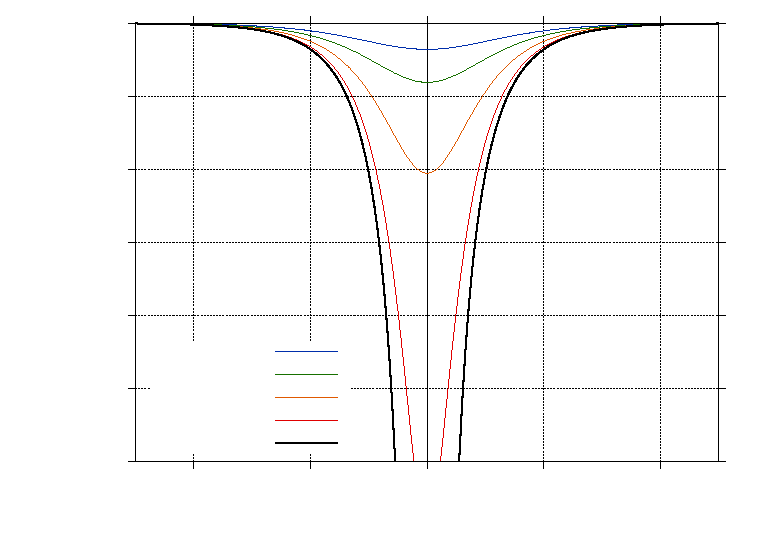
\includegraphics{Figures/twowires/InducedInteractionInterwireRealSpace/InducedInteraction}}%
    \gplfronttext
  \end{picture}%
\endgroup
  
\caption{The zero frequency potential $\tilde{V}_{FF,12}^\text{ind}(x,0)$ plotted as a function of $x$. The induced interaction is seen to increase with decreasing distance $d$. Parameters: $(n_Ba_B^3)^{1/3} = 0.01$, $(n_Ba_{BF}^3)^{1/3} = 0.1$, $l_t = 0$, $\frac{m_B}{m_F} = 7/40$, $\frac{n_F}{n_B^{1/3}} = 0.215$, $\frac{m_F^2}{m_B^2}\frac{n_B}{n_F^3} k_Fa_B = 22.10$.}  
\label{fig.VFF12indx}  
\end{center}    
\end{figure}

It is instructive to see, what the functional form of the induced interaction is; both in real and momentum space.  This is shown in figures \ref{fig.VFF12indq} and \ref{fig.VFF12indx}. The plot is done for the same set of parameters as in chapter \ref{Chapter5} for the analysis of the pairing. For this set of parameters one can calculate, that the range of the induced interaction in real space is approximately $1/k_F$: $k_F\xi \approx 1$. From figure \ref{fig.VFF12indx} it is then evident, that when the distance between the planes is on approximately the range of the interaction, $d\approx \xi$, the ratio of the induced interaction to the Fermi energy is approximately unity: $\tilde{V}_{FF,12}^\text{ind}(x=0,0)/\epsilon_{F,0} \approx 1$. This indicates, that when $d \approx \xi$, the interaction between the wires will start to be significant, which is physically reasonable.  




